\documentclass[avery5371]{flashcards}

\usepackage{amssymb}
\usepackage{amsmath}
\usepackage{datetime}
\usepackage{ragged2e} % \justify

\usepackage{hyperref}
\hypersetup{
    colorlinks=false,
}
\usepackage{graphicx}
\graphicspath{{./images/}}
\usepackage[export]{adjustbox}
\usepackage{lipsum}

\usepackage{tikz}
\usepackage{background}
\usepackage{wallpaper}
% ------ CUSTOM PATTERN ------- %
% defining the new dimensions
\newlength{\starsize}
\newlength{\starspread}
% declaring the keys in tikz
\tikzset{starsize/.code={\setlength{\starsize}{#1}},
    starspread/.code={\setlength{\starspread}{#1}}}
% setting the default values
\tikzset{starsize=1mm,starspread=3mm}
% declaring the pattern
\pgfdeclarepatternformonly[\starspread,\starsize]% variables
    {custom fivepointed stars}% name
    {\pgfpointorigin}% lower left corner
    {\pgfqpoint{\starspread}{\starspread}}% upper right corner
    {\pgfqpoint{\starspread}{\starspread}}% tilesize
    {% shape description
    \pgftransformshift{\pgfqpoint{\starsize}{\starsize}}
    \pgfpathmoveto{\pgfqpointpolar{18}{\starsize}}
    \pgfpathlineto{\pgfqpointpolar{162}{\starsize}}
    \pgfpathlineto{\pgfqpointpolar{306}{\starsize}}
    \pgfpathlineto{\pgfqpointpolar{90}{\starsize}}
    \pgfpathlineto{\pgfqpointpolar{234}{\starsize}}
    \pgfpathclose%
    \pgfusepath{fill}
    }
% defining the new dimensions
\newlength{\dotsize}
\newlength{\dotspread}
% declaring the keys in tikz
\tikzset{dotsize/.code={\setlength{\dotsize}{#1}},
    dotspread/.code={\setlength{\dotspread}{#1}}}
% setting the default values
\tikzset{dotsize=1mm,dotspread=1mm}
\pgfdeclarepatternformonly[\dotsize,\dotspread]%
    {custom dots}% name
    {\pgfqpoint{-\dotsize}{-\dotsize}} % lower left
    {\pgfqpoint{\dotsize}{\dotsize}} % upper right corner
    {\pgfqpoint{\dotspread}{\dotspread}}% tilesize
    {% shape description
      \pgfpathcircle{\pgfpoint{0}{0}}{\dotsize}
      \pgfusepath{fill}
    }

% ------ CUSTOM PATTERN ------- %

\usepackage{changepage}
\strictpagecheck
\usepackage[outline]{contour}
\contourlength{1pt}
\usetikzlibrary{patterns,calc}


\usepackage{geometry}
 \geometry{
 % --- PAPER SIZE --- %
 a4paper,
 hmargin=1.8mm,
 top=0cm,
 bottom=0cm,
 }

% --- FONT SIZE --- %
\cardfrontstyle[\small\slshape]{headings}
\cardbackstyle[\small]{empty}
% --- CARD SIZE --- %
\def\pageheight{7.4cm}
\def\pagewidth{9.5cm}
\renewcommand{\cardpapermode}{portrait}
\renewcommand{\cardrows}{4}
\renewcommand{\cardcolumns}{2}
\setlength{\cardheight}{\pageheight}
\setlength{\cardwidth}{\pagewidth}

\setlength{\cardmargin}{2mm}
\setlength{\topoffset}{0mm}
\setlength{\oddoffset}{0.1mm}
\setlength{\evenoffset}{0.1mm}
 
%%%% IMAGE DE FOND %%%%%
\newcommand{\bgimage}[2]{
\begin{tikzpicture}[remember picture, overlay]
    \filigrane
\end{tikzpicture}
}
\newcommand{\filigrane}{
    \checkoddpage
    \ifoddpage
        %\fill[opacity=0.1,pattern=custom fivepointed stars, starspread=3mm, starsize=0.75mm] (-0.49\paperwidth,-0.49\paperheight) rectangle (0.49\paperwidth,0.49\paperheight);
        \fill[opacity=0.1,pattern=custom dots, dotsize=0.15mm, dotspread=0.8mm] (-0.495\paperwidth,-0.495\paperheight) rectangle (0.495\paperwidth,0.495\paperheight);
    \else
        \fill[opacity=0.1,pattern=custom dots, dotsize=0.15mm, dotspread=0.8mm] (-0.495\paperwidth,-0.495\paperheight) rectangle (0.495\paperwidth,0.495\paperheight);
    \fi
}
\SetBgScale{1.0}% Select scale factor of logo
\SetBgAngle{0.0}% Select roation of logo
\SetBgOpacity{0.5}% Select opacity
\SetBgContents{\bgimage{1}{background_mathematiques}}% Set tikz picture
%\SetBgPosition{current page.north west}% Select location

\begin{document}

\TileWallPaper{10cm}{7cm}{background/background_biologie.png}
%\wpXoffset and \wpYoffset
\setlength{\wpXoffset}{1mm}
\setlength{\wpYoffset}{-7mm}
%%%%%%%%%%%%%%% TEMPLATE STANDARD %%%%%%%%%%%%%%%%
% --- background_MATIERE --- %
\SetBgContents{\bgimage{1}{background_biologie}}% Set tikz picture 
\cardfrontfoot{\begin{center}\rule{8cm}{0.1mm}\\ \textit{Niveau de complexité}\end{center}}
\begin{flashcard}[\begin{center}Matière -- L0\\ Thème\\\rule{8cm}{0.1mm}\end{center}]{
%%%%%%%%%%%%%%% ÉNONCÉ %%%%%%%%%%%%%%%%
\justify
\'Enoncé
\begin{enumerate}
    \item Réponse 1
    \item Réponse 2
    \item Réponse 3
	\item Réponse 4
\end{enumerate}
}
%%%%%%%%%%%%%%% ÉNONCÉ %%%%%%%%%%%%%%%%
\vspace*{\stretch{1}}
%%%%%%%%%%%%%%% RÉPONSE %%%%%%%%%%%%%%%%
\justify
\lipsum[2]
%%%%%%%%%%%%%%% RÉPONSE %%%%%%%%%%%%%%%%
\vspace*{\stretch{1}}
\end{flashcard}
%%%%%%%%%%%%%%% TEMPLATE STANDARD %%%%%%%%%%%%%%%%


%%%%%%%%%%%%%%% TEMPLATE IMAGE ENONCE + QR CODE REPONSE %%%%%%%%%%%%%%%%
% --- background_MATIERE --- %
\SetBgContents{\bgimage{1}{background_biologie}}% Set tikz picture 
\cardfrontfoot{\begin{center}\rule{8cm}{0.1mm}\\ \textit{Niveau de complexité}\end{center}}
\begin{flashcard}[\begin{center}Matière -- L0\\ Thème\\\rule{8cm}{0.1mm}\end{center}]{
%%%%%%%%%%%%%%% ÉNONCÉ %%%%%%%%%%%%%%%%
\justify
\begin{minipage}[c]{0.6\linewidth}
    \'Enoncé
    \begin{enumerate}
        \item Réponse 1
        \item Réponse 2
        \item Réponse 3
    	\item Réponse 4
    \end{enumerate}
\end{minipage}%
\hfill
\begin{minipage}[c]{0.3\linewidth}
    \strut\vspace*{-\baselineskip}\newline
    
\includegraphics[max size={\textwidth}{0.5\textheight}, center, keepaspectratio]{QCM/MATIERE/ID_QUESTION/placeholder_150.png}
\end{minipage}
}
%%%%%%%%%%%%%%% ÉNONCÉ %%%%%%%%%%%%%%%%
\vspace*{\stretch{1}}
%%%%%%%%%%%%%%% RÉPONSE %%%%%%%%%%%%%%%%
\justify
Nam dui ligula, fringilla a, euismod sodales, sollicitudin vel, wisi.
Morbi auctor lorem non justo. Nam lacus libero, pretium at, lobortis vitae, ultricies et, tellus. Donec aliquet, tortor sed accumsan
bibendum, erat ligula aliquet magna, vitae ornare odio metus a
mi. Morbi ac orci et nisl hendrerit mollis. Suspendisse ut massa.
Cras nec ante. Pellentesque a nulla. Cum sociis natoque penatibus
et magnis dis parturient montes, nascetur ridiculus mus. Aliquam
tincidunt urna. Nulla ullamcorper vestibulum turpis. Pellentesque
cursus luctus mauris.
\newline

\includegraphics[max size={\textwidth}{0.2\textheight}, center, keepaspectratio]{QCM/MATIERE/ID_QUESTION/qrcode.png}

%%%%%%%%%%%%%%% RÉPONSE %%%%%%%%%%%%%%%%
\vspace*{\stretch{1}}
\end{flashcard}
%%%%%%%%%%%%%%% TEMPLATE IMAGE ENONCE + QR CODE REPONSE%%%%%%%%%%%%%%%%

%%%%%%%%%%%%%%%%%%%%%%%%%%%%%%%%%%%%%%%%%%%%%%%%%%%%%%%%%%%%%%%%%%%%
% --- background_MATIERE --- %
\SetBgContents{\bgimage{1}{background_physique}}% Set tikz picture 
\cardfrontfoot{\begin{center}\rule{8cm}{0.1mm}\\ \textit{Comprendre, appliquer}\end{center}}
\begin{flashcard}[\begin{center}Physique -- L0\\ Lois de Newton et Kepler et leurs applications\\\rule{8cm}{0.1mm}\end{center}]{
%%%%%%%%%%%%%%% ÉNONCÉ %%%%%%%%%%%%%%%%
\justify
Pour un point matériel en mouvement uniforme (c'est-à-dire un mouvement au cours duquel la norme de la vitesse est constante) :
    \begin{enumerate}
        \item le principe d'inertie est vérifié.
        \item la trajectoire est rectiligne.
        \item la trajectoire peut être un cercle.
    	\item la somme des forces qui s'exercent sur le corps est nulle
    \end{enumerate}
}
%%%%%%%%%%%%%%% ÉNONCÉ %%%%%%%%%%%%%%%%
\vspace*{\stretch{1}}
%%%%%%%%%%%%%%% RÉPONSE %%%%%%%%%%%%%%%
\justify
Principe d'inertie : Dans un référentiel galiléen, si un système assimilé à un point matériel n'est soumis à aucune force – système isolé – ou s'il est soumis à un ensemble de forces de résultante nulle ($\Sigma\vec{F}_{ext}=\vec{0}$) – système pseudo-isolé – alors il est immobile ou animé d'un mouvement rectiligne uniforme.

Dans cette question, il s'agit de faire la distinction entre mouvement uniforme (la norme de la vitesse est constante, on ne sait rien de la trajectoire) et mouvement rectiligne uniforme ou mouvement circulaire uniforme (norme de la vitesse constante et trajectoire fixée).

Vous pouvez retrouver ces éléments dans la ressource suivante :
\newline

\includegraphics[max size={\textwidth}{0.2\textheight}, center, keepaspectratio]{QCM/Physique/UTC-001/qrcode.png}
%%%%%%%%%%%%%%% RÉPONSE %%%%%%%%%%%%%%%%
\vspace*{\stretch{1}}
\end{flashcard}

\cardfrontfoot{\begin{center}\rule{8cm}{0.1mm}\\ \textit{Changement de langage}\end{center}}
\begin{flashcard}[\begin{center}Physique -- L0\\ Optique géométrique\\\rule{8cm}{0.1mm}\end{center}]{
%%%%%%%%%%%%%%% ÉNONCÉ %%%%%%%%%%%%%%%%
\justify

\begin{minipage}[c]{0.6\linewidth}
    Étant donné le sens de propagation de la lumière choisi et indiqué sur le schéma, si $A$ est la position de l'objet, $A'$ celle de l'image et $O$ le centre de la lentille convergente, alors :
    \begin{enumerate}
        \item $\overline{OA}$ est positif et $\overline{OA'}$ est négatif.
        \item $\overline{OA}$ est négatif et $\overline{OA'}$ est positif.
        \item $\overline{OA}$ et $\overline{OA'}$ sont négatifs.
    	\item $\overline{OA}$ et $\overline{OA'}$ sont positifs.
    \end{enumerate}
\end{minipage}%
\hfill
\begin{minipage}[c]{0.3\linewidth}
    \strut\vspace*{-\baselineskip}\newline
    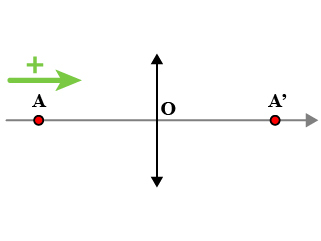
\includegraphics[max size={\textwidth}{0.9\textheight}, center, keepaspectratio]{QCM/Physique/UTC-002/lentille.jpg}
\end{minipage}
}
%%%%%%%%%%%%%%% ÉNONCÉ %%%%%%%%%%%%%%%%
\vspace*{\stretch{1}}
%%%%%%%%%%%%%%% RÉPONSE %%%%%%%%%%%%%%%%
\justify
Attention, ici on utilise les mesures algébriques, dont le signe dépend du point initial (ici $O$) et du point final ($A$ ou $A'$). Ici le sens allant de la gauche vers la droite est pris comme positif.

Vous pouvez revoir le cours en suivant le lien donné par le QR Code ci-dessous.
\newline

\includegraphics[max size={\textwidth}{0.2\textheight}, center, keepaspectratio]{QCM/Physique/UTC-002/qrcode.png}

%%%%%%%%%%%%%%% RÉPONSE %%%%%%%%%%%%%%%%
\vspace*{\stretch{1}}
\end{flashcard}

\SetBgContents{\bgimage{1}{background_mathematiques}}% Set tikz picture 
\cardfrontfoot{\begin{center}\rule{8cm}{0.1mm}\\ \textit{Comprendre, appliquer}\end{center}}
\begin{flashcard}[\begin{center}Mathématiques -- L0\\ Statistiques\\\rule{8cm}{0.1mm}\end{center}]{
%%%%%%%%%%%%%%% ÉNONCÉ %%%%%%%%%%%%%%%%
\justify

\begin{minipage}[c]{0.6\linewidth}
On considère une série statistique à 13 éléments décrite par sa courbe des fréquences cumulées croissantes.

Lequel des graphiques suivant peut correspondre à son histogramme (en fréquence) ?
    \begin{enumerate}
        \item Dessin de gauche
        \item Dessin du milieu
    	\item Dessin de droite
    \end{enumerate}
\end{minipage}%
\hfill
\begin{minipage}[c]{0.3\linewidth}
    \strut\vspace*{-\baselineskip}\newline
    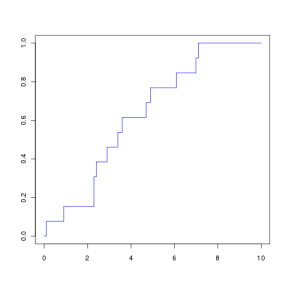
\includegraphics[max size={\textwidth}{0.5\textheight}, center, keepaspectratio]{QCM/Mathematiques/UTC-052/freq_cumulees.png}
    \includegraphics[max size={\textwidth}{0.5\textheight}, center, keepaspectratio]{QCM/Mathematiques/UTC-052/histo_fréq.png}
\end{minipage}
}
%%%%%%%%%%%%%%% ÉNONCÉ %%%%%%%%%%%%%%%%
\vspace*{\stretch{1}}
%%%%%%%%%%%%%%% RÉPONSE %%%%%%%%%%%%%%%%
\justify
D'après le graphe des fréquences cumulées, le minimum de la série est proche de 0.

Le maximum de la série associée au dessin du milieu est supérieur à 8; ce ne peut donc être la bonne réponse.

Il n'y a aucun élément entre 2 et 4 dans la série associée au diagramme de gauche; ce ne peut donc être la bonne réponse.

Le dessin de droite correspond à la série initiale.
%%%%%%%%%%%%%%% RÉPONSE %%%%%%%%%%%%%%%%
\vspace*{\stretch{1}}
\end{flashcard}

\cardfrontfoot{\begin{center}\rule{8cm}{0.1mm}\\ \textit{Comprendre, appliquer}\end{center}}
\begin{flashcard}[\begin{center}Mathématiques -- L0\\ Statistiques\\\rule{8cm}{0.1mm}\end{center}]{
%%%%%%%%%%%%%%% ÉNONCÉ %%%%%%%%%%%%%%%%
\justify

\begin{minipage}[c]{0.6\linewidth}
On considère une série statistique à 13 éléments décrite par sa courbe des fréquences cumulées croissantes.

Lequel des graphiques suivant peut correspondre à son histogramme (en fréquence) ?
    \begin{enumerate}
        \item Dessin de gauche
        \item Dessin du milieu
    	\item Dessin de droite
    \end{enumerate}
\end{minipage}%
\hfill
\begin{minipage}[c]{0.3\linewidth}
    \strut\vspace*{-\baselineskip}\newline
    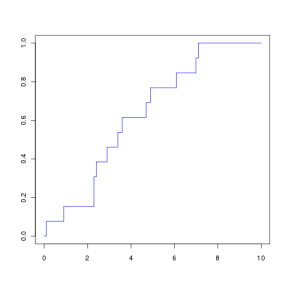
\includegraphics[max size={\textwidth}{0.5\textheight}, center, keepaspectratio]{QCM/Mathematiques/UTC-052/freq_cumulees.png}
    \includegraphics[max size={\textwidth}{0.5\textheight}, center, keepaspectratio]{QCM/Mathematiques/UTC-052/histo_fréq.png}
\end{minipage}
}
%%%%%%%%%%%%%%% ÉNONCÉ %%%%%%%%%%%%%%%%
\vspace*{\stretch{1}}
%%%%%%%%%%%%%%% RÉPONSE %%%%%%%%%%%%%%%%
\justify
D'après le graphe des fréquences cumulées, le minimum de la série est proche de 0.

Le maximum de la série associée au dessin du milieu est supérieur à 8; ce ne peut donc être la bonne réponse.

Il n'y a aucun élément entre 2 et 4 dans la série associée au diagramme de gauche; ce ne peut donc être la bonne réponse.

Le dessin de droite correspond à la série initiale.
%%%%%%%%%%%%%%% RÉPONSE %%%%%%%%%%%%%%%%
\vspace*{\stretch{1}}
\end{flashcard}

\cardfrontfoot{\begin{center}\rule{8cm}{0.1mm}\\ \textit{Comprendre, appliquer}\end{center}}
\begin{flashcard}[\begin{center}Mathématiques -- L0\\ Statistiques\\\rule{8cm}{0.1mm}\end{center}]{
%%%%%%%%%%%%%%% ÉNONCÉ %%%%%%%%%%%%%%%%
\justify

\begin{minipage}[c]{0.6\linewidth}
On considère une série statistique à 13 éléments décrite par sa courbe des fréquences cumulées croissantes.

Lequel des graphiques suivant peut correspondre à son histogramme (en fréquence) ?
    \begin{enumerate}
        \item Dessin de gauche
        \item Dessin du milieu
    	\item Dessin de droite
    \end{enumerate}
\end{minipage}%
\hfill
\begin{minipage}[c]{0.3\linewidth}
    \strut\vspace*{-\baselineskip}\newline
    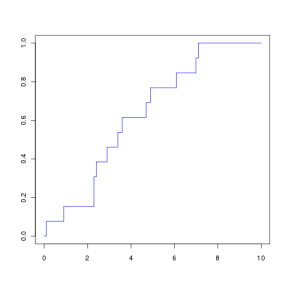
\includegraphics[max size={\textwidth}{0.5\textheight}, center, keepaspectratio]{QCM/Mathematiques/UTC-052/freq_cumulees.png}
    \includegraphics[max size={\textwidth}{0.5\textheight}, center, keepaspectratio]{QCM/Mathematiques/UTC-052/histo_fréq.png}
\end{minipage}
}
%%%%%%%%%%%%%%% ÉNONCÉ %%%%%%%%%%%%%%%%
\vspace*{\stretch{1}}
%%%%%%%%%%%%%%% RÉPONSE %%%%%%%%%%%%%%%%
\justify
D'après le graphe des fréquences cumulées, le minimum de la série est proche de 0.

Le maximum de la série associée au dessin du milieu est supérieur à 8; ce ne peut donc être la bonne réponse.

Il n'y a aucun élément entre 2 et 4 dans la série associée au diagramme de gauche; ce ne peut donc être la bonne réponse.

Le dessin de droite correspond à la série initiale.
%%%%%%%%%%%%%%% RÉPONSE %%%%%%%%%%%%%%%%
\vspace*{\stretch{1}}
\end{flashcard}

\cardfrontfoot{\begin{center}\rule{8cm}{0.1mm}\\ \textit{Comprendre, appliquer}\end{center}}
\begin{flashcard}[\begin{center}Mathématiques -- L0\\ Statistiques\\\rule{8cm}{0.1mm}\end{center}]{
%%%%%%%%%%%%%%% ÉNONCÉ %%%%%%%%%%%%%%%%
\justify

\begin{minipage}[c]{0.6\linewidth}
On considère une série statistique à 13 éléments décrite par sa courbe des fréquences cumulées croissantes.

Lequel des graphiques suivant peut correspondre à son histogramme (en fréquence) ?
    \begin{enumerate}
        \item Dessin de gauche
        \item Dessin du milieu
    	\item Dessin de droite
    \end{enumerate}
\end{minipage}%
\hfill
\begin{minipage}[c]{0.3\linewidth}
    \strut\vspace*{-\baselineskip}\newline
    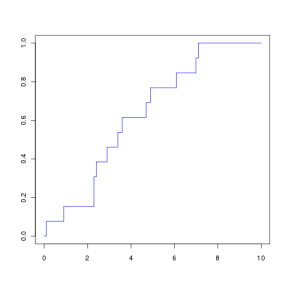
\includegraphics[max size={\textwidth}{0.5\textheight}, center, keepaspectratio]{QCM/Mathematiques/UTC-052/freq_cumulees.png}
    \includegraphics[max size={\textwidth}{0.5\textheight}, center, keepaspectratio]{QCM/Mathematiques/UTC-052/histo_fréq.png}
\end{minipage}
}
%%%%%%%%%%%%%%% ÉNONCÉ %%%%%%%%%%%%%%%%
\vspace*{\stretch{1}}
%%%%%%%%%%%%%%% RÉPONSE %%%%%%%%%%%%%%%%
\justify
D'après le graphe des fréquences cumulées, le minimum de la série est proche de 0.

Le maximum de la série associée au dessin du milieu est supérieur à 8; ce ne peut donc être la bonne réponse.

Il n'y a aucun élément entre 2 et 4 dans la série associée au diagramme de gauche; ce ne peut donc être la bonne réponse.

Le dessin de droite correspond à la série initiale.
%%%%%%%%%%%%%%% RÉPONSE %%%%%%%%%%%%%%%%
\vspace*{\stretch{1}}
\end{flashcard}
\end{document}


